\documentclass[12pt, twoside]{article}
\documentclass[12pt, twoside]{article}
\usepackage[letterpaper, margin=1in, headsep=0.2in]{geometry}
\setlength{\headheight}{0.6in}
%\usepackage[english]{babel}
\usepackage[utf8]{inputenc}
\usepackage{microtype}
\usepackage{amsmath}
\usepackage{amssymb}
%\usepackage{amsfonts}
\usepackage{siunitx} %units in math. eg 20\milli\meter
\usepackage{yhmath} % for arcs, overparenth command
\usepackage{tikz} %graphics
\usetikzlibrary{quotes, angles}
\usepackage{graphicx} %consider setting \graphicspath{{images/}}
\usepackage{parskip} %no paragraph indent
\usepackage{enumitem}
\usepackage{multicol}
\usepackage{venndiagram}

\usepackage{fancyhdr}
\pagestyle{fancy}
\fancyhf{}
\renewcommand{\headrulewidth}{0pt} % disable the underline of the header
\raggedbottom
\hfuzz=2mm %suppresses overfull box warnings

\usepackage{hyperref}
\usepackage{float}

\title{Algebra 2}
\author{Chris Huson}
\date{October 2023}

\fancyhead[LE]{\thepage}
\fancyhead[RO]{\thepage \\ Name: \hspace{4cm} \,\\}
\fancyhead[LO]{BECA / Huson / Algebra 2: Sequences and functions \\* 11 October 2023}

\begin{document}

\subsubsection*{1.13 PreTest2: Graphing sequences}
\begin{enumerate}

\item A sequence $f$ is shown below as a graph and as a table.
\begin{multicols}{2}
\begin{center}
    \begin{tikzpicture}[yscale=0.4]
        \draw [thin, color=lightgray, xstep=0.5cm,ystep=2.0cm] (0,0) grid (5,18);
        \foreach \x in {0,1,2,...,5}
        \draw (\x cm,3pt) -- (\x cm,-3pt) node[below] {$\x$};
        \foreach \y in {0,2,...,18}
        \draw[shift={(0,\y)},color=black] (2pt,0pt) -- (-2pt,0pt) node[left]  {$\y$};
        \draw [thick, ->] (0,0) -- (+5.4,0) node [above right] {$n$};
        \draw [thick, ->] (0,0) -- (0,18.4) node [above right] {$f(n)$};
        \node at (0,16){$\bullet$};
        \node at (1,8){$\bullet$};
        \node at (2,4){$\bullet$};
        \node at (3,2){$\bullet$};
        \node at (4,1){$\bullet$};
        %\draw [thick, <->,smooth,domain=-0.5:8.5] plot(\x,-\x*\x+8*\x);
    \end{tikzpicture}
    \end{center}
    \begin{tabular}{c|c}
        $n$ & $f(n)$ \\ \hline
        0 & 16 \\ 
        1 & 8 \\ 
        2 & 4 \\ 
        3 & 2 \\ 
        4 & 1 \\ 
        \end{tabular}
    \end{multicols}
    \begin{enumerate}
        \item Is sequence $f$ geometric or arithmetic? Explain how you know. \vspace{2cm}
        \item Write an equation to define sequence $f$ recursively. \vspace{3cm}
        \item For term $f(n)$, what are some values of $n$ that make sense to use? What are some values of $n$ that don't make sense to use? Explain your reasoning.
    \end{enumerate}

\newpage
\item An arithmetic sequence $A$ is shown below in the table.
    \begin{multicols}{2}
        \renewcommand{\arraystretch}{2}
        \begin{table}[H]
        \begin{tabular}{c|c}
            $n$ & $A(n)$ \\ \hline
            1 & $\displaystyle \frac{7}{2}$ \\ 
            2 & ? \\ 
            3 & $\displaystyle \frac{13}{2}$ \\ 
            4 & 8 \\ 
            5 & ? \\ 
        \end{tabular}
    \end{table} \vspace{2cm}
    \columnbreak
        \begin{tikzpicture}[yscale=0.8]
            \draw [thin, color=lightgray, xstep=0.5cm,ystep=0.5cm] (0,0) grid (5,10);
            \foreach \x in {0,1,2,...,5}
            \draw (\x cm,3pt) -- (\x cm,-3pt) node[below] {$\x$};
            \foreach \y in {0,1,...,10}
            \draw[shift={(0,\y)},color=black] (2pt,0pt) -- (-2pt,0pt) node[left]  {$\y$};
            \draw [thick, ->] (0,0) -- (+5.4,0);
            \draw [thick, ->] (0,0) -- (0,10.4);
        \end{tikzpicture}
    \end{multicols}
    \begin{enumerate}[itemsep=1cm]
        \item What is the rate of change, the constant difference $d$?
        \item Find the missing values. \\[0.5cm]
            $A(2)=$ \\[0.5cm] 
            $A(5)=$
        \item Plot the sequence on the grid above.
        \item Write a recursive definition for sequence $A$.
    \end{enumerate}

\newpage
\item Here are two sequences:
    \begin{multicols}{2}
        Sequence A
        \renewcommand{\arraystretch}{2}
        \begin{table}[H]
        \begin{tabular}{c|c}
            term number & value \\ \hline
            0 & $\displaystyle \frac{1}{9}$ \\ 
            1 & $\displaystyle \frac{1}{3}$ \\ 
            2 & 1 \\ 
            3 & 3 \\ 
            4 & 9 \\ 
        \end{tabular}
    \end{table} \vspace{2cm}
    \columnbreak
    Sequence B \\
        \begin{tikzpicture}[yscale=0.1]
            \draw [thin, color=lightgray, xstep=0.5cm,ystep=5.0cm] (0,0) grid (5,50);
            \foreach \x in {0,1,2,...,5}
            \draw (\x cm,3pt) -- (\x cm,-3pt) node[below] {$\x$};
            \foreach \y in {0,10,...,50}
            \draw[shift={(0,\y)},color=black] (2pt,0pt) -- (-2pt,0pt) node[left]  {$\y$};
            \draw [thick, ->] (0,0) -- (+5.4,0);
            \draw [thick, ->] (0,0) -- (0,53.4);
            \node at (0,10){$\bullet$};
            \node at (1,20){$\bullet$};
            \node at (2,30){$\bullet$};
            \node at (3,40){$\bullet$};
            \node at (4,50){$\bullet$};
        \end{tikzpicture}
    \end{multicols}
    \begin{enumerate}[itemsep=1.5cm]
        \item For sequence $A$, describe a way to produce each new term from the previous term.
        \item For sequence $B$, describe a way to produce each new term from the previous term.
        \item Write a definition for the $n^{th}$ term of sequence $A$. (an explicit formula, not a recursive one)
        \item Write a definition for the $n^{th}$ term of sequence $B$.
        \item If these sequences continue, then which is greater, $A$ or $B$? Explain or show how you know.
    \end{enumerate}

\newpage
\item The first few terms of a geometric sequence $B$ are shown in the table.
\begin{multicols}{2}
    \renewcommand{\arraystretch}{2}
    \hspace{1cm}
    \begin{tabular}{c|c}
        $n$ & $B(n)$ \\ \hline
        0 & $\displaystyle \frac{2}{3}$ \\ 
        1 & $-1$ \\ 
        2 & $\displaystyle \frac{3}{2}$ \\ 
        3 & $\displaystyle -\frac{9}{4}$ \\ 
        4 & ? \\ 
    \end{tabular}
    \begin{enumerate}[itemsep=1cm]
        \item What is the growth rate, the constant ratio $r$?
        \item Find $B(4)=$
        \item Write a recursive definition for sequence $B$.
    \end{enumerate}
\end{multicols} \vspace{1cm}

\item An arithmetic sequence has terms $h(1)=-2$ and $h(5)=10$.
    \begin{enumerate}
        \item What is the common difference, $d$? \vspace{2cm}
        \item Write a formula for the $n^{th}$ term, $h(n)$. \vspace{2cm}
        \item What is the value of $n$ when $h(n)=22$?
    \end{enumerate} \vspace{2cm}

\item A geometric sequence has terms $\displaystyle j(0)=\frac{16}{9}$ and $j(2)=1$. Find $j(3)$.


\end{enumerate}
\end{document}